\documentclass{article}
\usepackage[T1]{fontenc}
\usepackage{lmodern}
\usepackage{graphicx}
\usepackage{amsmath,amssymb}
\usepackage[a4paper,margin=2cm]{geometry}
\usepackage[absolute,overlay]{textpos}
\setlength{\TPHorizModule}{1mm}
\setlength{\TPVertModule}{1mm}
\usepackage[indonesian]{babel}
\usepackage{hyperref}
\setlength{\emergencystretch}{2em}
% unit: Halaman 28

\begin{document}

% === Halaman 28 (llm) ===

\vspace{193.05mm}

\vspace{60mm}
Sebaran titik di dalam kurva eliptik $y^2 = x^3 + x + 6 \pmod{11}$ pada $\text{GF}(11)$

% deskripsi: Grafik sebaran titik (scatter plot) dari persamaan kurva eliptik $y^2 = x^3 + x + 6 \pmod{11}$ pada bidang koordinat dengan sumbu x dari 0 sampai 10 dan sumbu y dari 0 sampai 10.
% bbox normalisasi: [0.2000, 0.1000, 0.7500, 0.7500]
\begin{textblock*}{115.50mm}(42.00mm,29.70mm)
\noindent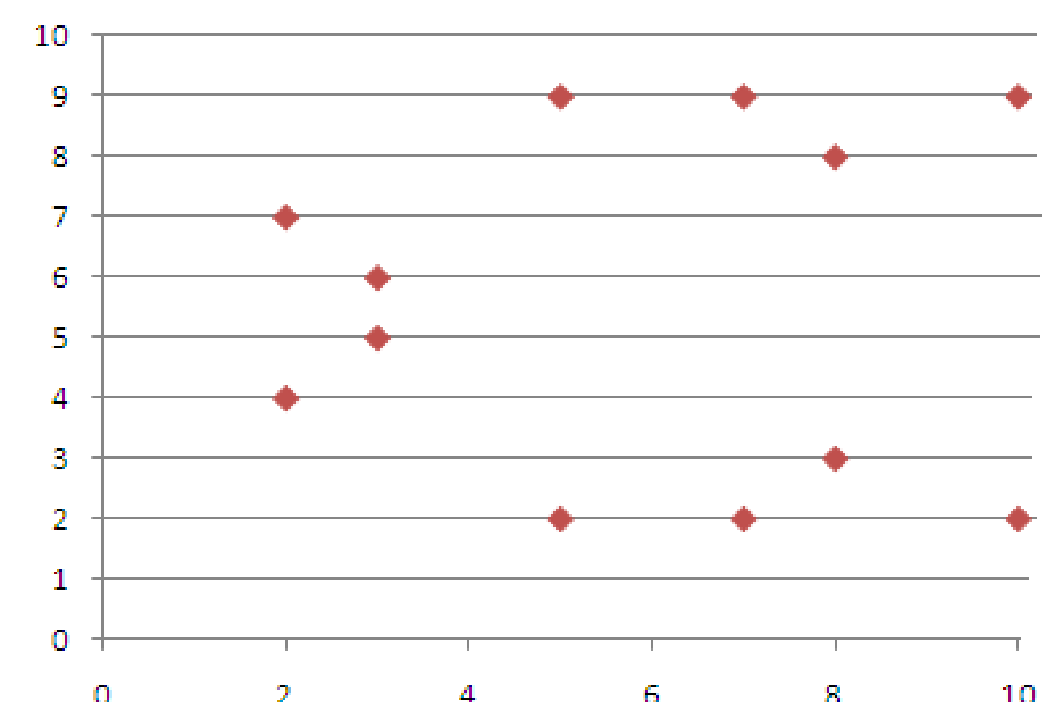
\includegraphics[width=115.50mm,height=193.05mm]{../../images/llm/page_028_img_01.png}%
\end{textblock*}

\end{document}
